\chapter{The Framework}

This chapter describes all of the choices considered for the framework. It will describe how the game influenced the server and framework, and advantages and disadvantages of this. The chapter focuses on the separation of the framework and the game - it will describe the relationship between different game functions and their framework counterpart. It will also describe the implementation of the said features and the possible uses of it. In the end, the test andits results will be described.

\section{Design}\label{sec:desFram}
With the prototyping described in \Cref{sec:game} we can design a server architecture to accommodate the described features. In this section we will first describe the overall architecture and then look at the individual components.
\subsection{Server Architecture}
\label{sec:server}

The server is structured in three layers: a dispatcher service, a logic layer and a data layer. Because we wanted to develop a framework for creating future location-based games, we had to make a decision how to achieve this goal. We could not interleave framework-specific functionality with the specific game we developed along side our framework. The result was these three layers. We wanted to build a communication layer to handle the interface between the client and the server and a data layer to handle the interface between the server and the database. These two layers were chosen rather intuitively early in the design process. Our next choice was how to choose a way to implement a specific game capable of using the framework, while still being scalable and encapsulated. We decided to make the threaded class called Game Thread handle all game-specific calculations, logics and responses. 
It was helpful to build a game alongside the framework, this helped us to figure out the need for a service to handle timed events in the framework, which resulted in the Event Timer. We also discovered the need for unit to handle client requests that requested functionality prior to the Game Thread. This was requests like logging in, and seeing all active games, which cannot be handled by a game thread yet since it might not be created yet. The result was the Admin. The Event Timer and the Admin are both positioned in the Logic Layer, because they help make logical decisions based on requests made by the client. 

%Server Architecture
\paragraph{Dispatcher Service}
The dispatcher is a service responsible for handling the communication with the client. It consists of an asynchronous I/O\fixme{IO or I/O throughout report?} and the dispatcher itself. Communication is done by an XML interface where requests from the client is verified by the dispatcher and passed to either the Admin module or a Game Thread depending on the message. 

\paragraph{Logic Layer}
This layer represents the business logic of the server application. The Admin module handles user creation, user login and game creation and is general for all game implementations. Game Thread is where specific game logic is implemented and its implementation will vary depending on the type of game. Event Timer is a general module handling events specified to happen at certain times. The game threads are responsible for creating events for themselves. The event timer will then notify a game thread at the specified time. As illustrated in \cref{fig:serverarch}, game threads are not a part of the framework, but can be ``plugged in''\fixme{change word??} to the framework. This increases the versatility of the game threads, since a developer can create his own game threads and plug them into the framework.

\paragraph{Data Layer}
Is the database representation in the model using the data mapper pattern\fxwarning{WE book ref}. The gateway is responsible for querying and updating the database and mapping the tables to objects used in the game logic and administration.

\begin{figure}[H]
  \centering
  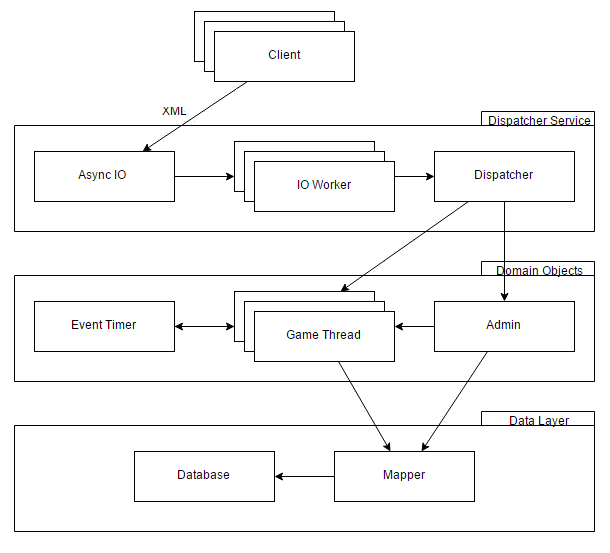
\includegraphics[width=\textwidth]{billeder/serverarch.png}  
  \caption{Architecture of server displaying the branching of an incoming connection}
  \label{fig:serverarch}
\end{figure}

%Dispatcher Service
\subsection{Dispatcher Service}
This layer is responsible for communication with the between client and server, this responsibility is divided between an IO module and a Dispatcher. In this section we will first examine Synchronous and Asynchronous IO in order to determine which is best suited for this framework and then the Dispatcher which forwards messages to the Logic Layer. We decided on Asynchronous IO and base our design on \cite{?} 	 %http://msdn.microsoft.com/en-us/library/fx6588te%28v=vs.110%29.aspx

The Asynchronous IO unit is handling socket creation and TCP/IP communication, a rather trivial part of a client-server interface when you disregard the communication type. The need for out Dispatcher unit has been revealed by building our game. We need a way to dispatch requests from the client to the right component and method on the server. We dispatch to either Admin or Game Thread, by reading the request from the client and determine what type of request it is and continue accordingly. We decided to build the Dispatcher to encapsulate reading and analysing the requests from the client. Alternatively, we could have handed everything to Admin and incorporated the Dispatcher's functionality into the Admin, but we did not consider this a well structured framework.

% ms-syn-asyn - http://msdn.microsoft.com/en-us/library/windows/desktop/aa365683(v=vs.85).aspx


\section{Synchronous vs. Asynchronous I/O}
%What is B/NB I/O?
I/O can be handled either synchronously or asynchronously. A synchronous I/O operation is blocking, i.e., the thread that executes the current job is in a waiting state, where it does not compute anything, until it gets a response. An asynchronous I/O operation is non-blocking and therefore allows the thread to execute another job while waiting for the I/O operation to finish. This is illustrated on \Cref{fig:syncasync}. The figure does not show the overhead caused by using asynchronous I/O, which causes this to not always be the best solution, especially if there are many short I/O operations \cite{ms-syn-asyn}.

\begin{figure}[H]
  \centering
  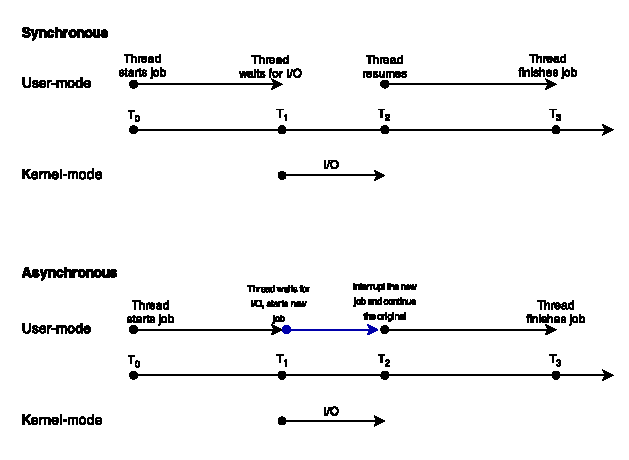
\includegraphics[scale=1.2]{billeder/sync-async.pdf}  
  \caption{Synchronous and asyncronous execution. Based on \cite{ms-syn-asyn}.}
  \label{fig:syncasync}
\end{figure}

This is the case for one or few users, but if there are many users at once they either have to wait in queue for previous I/O operations to finish, or each operation has to be executed in it's own thread, which would potentially result in many active threads, requiring a lot of memory. As pointed out by \citet{amir} it is worth noting that an asynchronous call that results in a synchronous operation causes the application to block, and therefore should be considered during implementation.

To enable the server to scale better, the I/O is implemented asynchronously. When the server receives an input, it is asynchronously sent to a dispatcher which sends it to the correct place; this is described in \Cref{sec:server}. Because of the many parts that have to interact, it is hard to determine if this implementation behaves as expected without testing it, but changing to a synchronous implementation would not be very expensive, as the asynchronous code is very similar to the synchronous code thanks to .NET's \texttt{Async} and \texttt{Await} keywords \cite{ms-asyn}. Making both implementations available at the same time, and letting the user choose which one to use, would also be relatively easy to do, but it adds some extra complexity to the code, as changes in one implementation would require similar changes in the other.
%What are the advantages and disadvantages?

%Which alternative(s) is/are there?

%Why did we make the choice we did?

%How flexible is it?
% - Could it easily be changed? 
% - Could both be implemented and the framework-user decides which one to use?
%
%\section{Synchronous vs. Asynchronous I/O}\fxfatal{This section will be rewritten with proper sources.}
%For the client/server socket communication, a choice between synchronous and asynchronous I/O has to be taken.
%% % blocking % %
%Synchronous I/O can have a better performance than asynchronous, but can cause problems when using a threaded architecture that spawns a new thread for each client. This is particularly true when the server should be scalable in regards to its number of connected clients. There might be 5 and there might be 5000 or even more.
%Tests show that threads are very efficient when it comes to memory and context switching, but only when the threads are kept alive for the entire execution of an application. This is not the case for our application, which will likely have many connections of varying durations during its up-time. \fixme{cite}\\\\
%% % non-blocking % %
%Asynchronous I/O is chosen for this project. It scales well when there are many clients, and the system should scale well with a potentially large number of clients. A notable advantage of asynchronous is that it limits the number of concurrent threads. The server asynchronously accepts a connection request from a client, and then starts an asynchronous worker thread to handle communication with the client. Meanwhile it continues to listen for new client connections.
%

%The ability to scale well does not come for free, however. Non-blocking IO is not always as fast as blocking IO and this can result in decreased performance. 
\subsection{Dispatcher}\label{subsec:dispatcherdesign}
The Dispatcher is a central component in the framework. It is placed in the \textit{Dispatcher Service} in the architecture, and is the first receiving to interpret a request sent by a client. The dispatcher simply dispatches a call to the appropriate method with the appropriate parameters when it receives XML data. In order to do this, it reads as little XML as possible to extract information to decide the appropriate destination and the right method to call. It attaches the entire XML as parameter to the method call.

The Dispatcher looks for the specified method call in the XML to hand it over to the Admin class. This is static calling of methods with attached XML. The Dispatcher waits for the Admin to return an XML, which it returns to the Async IO.

The Dispatcher handles all requests to a game thread dynamically, as it only interpret the method call before handing it over to the game thread. It then waits until the game thread returns a XML string, which it returns to the Async IO.

%Logic Layer
\subsection{Logic Layer}
This layer parses and reacts to the messages received from the Dispatcher. The logic layer interact with the Game Threads and consists of the Event Timer module which is callable from the Game Threads and can do a callback at a later time. The layer also contains the Admin module responsible for creating Game threads as well as non-game specifics such as authenticating logins.

The framework allows the user to use services like logging a client in through an XML-based interface. Services in the framework requires the user to implement proper XML-based communication on the client-side. A discussion about the use of XML seen in \fixme{ref til johans afsnit om valg af XML}. The framework also offers to handle Game Events, timed to occur after a specified time-stamp. This service used by creating a Game Event in the Game Thread being build by the user of the framework. We decided to build the Event Timer this way to encapsulate time-handling, and make a generic module that can be used for many different events. The user of the framework can specify what should happen for a given event in the Game Event class.

\subsubsection{Admin}\label{subsec:admindesign}
The Admin module is responsible for handling server-requests not related to specifict Game Threads. The Admin module handles administrative calls like creating new games or accounts as well as verifying login requests. 

%impl?
%A \textit{CreateGame} call cannot be send to a game thread, obviously because the game thread has not yet been created. Therefore this method will create a game from a model-class \textit{Game}, store it in the database with the provided settings, start a thread on the server for it to run on. 


\subsection{Event Timer}\label{subsec:eventtimerdesign}


%Game Block
\subsection{Game Block}
This is the workstation of the user of the framework. This block interacts with all the layers in the framework and makes use of the functionality provided by the framework. This class encapsulates all game-specific logic.

This is where we designed the framework to allow the user to develop a game. The framework has several rules the user has to follow when using the framework. They are explained for each module in the design. An example is the XML communication from client to server.
 
\subsection{Game thread-pool}
The game thread-pool is a collection of active game thread-instances, uniquely identified by a game-Id.

The game thread-pool is used as a handle to the game threads, and allows dynamic call to the desired game through method-parametrization. 

\subsection{Game thread}
\paragraph{Starting a game}
A game thread will be initialised and started when a user requests to host a game. A game will be assigned a game-id by the server, user-specified settings for hosting the game will be initialised and the game will be created in the database. 

When the server initialises each setting, it calls a method within the game thread-class. These methods calls the database-controller to change the state of the game in the database. These settings are:
\begin{itemize}
\item Game-privacy (Public or private game)
\item Number of teams
\item Game start-time
\item Game end-time
\item Game-boundary NorthWest GPS-coordinate
\item Game-boundary SouthEast GPS-coordinate
\end{itemize}

\paragraph{Updating a game}
Updates to a game can be split into two groups. One group is specific changes to a game, like inviting a new player or firing a gun. Another group is updating a players position when moving around in the game.

Updating a players position is trivial. The game thread receives a game-id, player-id and a new position. It calls the database-controller to store the new position in the database.

When performing an action like firing a gun, the server will have to fetch the gunman's position and the victim's position. It will then calculate if the range of the fired weapon allows the victim to be hit. If the shot is successful it will return that to the player, if the shot is unsuccessful it will return that the victim is out of range. 

All updates to change the state of a game will be in the game thread-class. This class will need to contain methods for all the in-game functionality. 

\paragraph{Closing a game}
When a game ends, the call will come from the timer thread. This will ask the game thread to clean up what is has stored in the database, and return a status message. The timer thread will then continue to close the game thread. 

%Data Layer
\subsection{Data Layer}
The data layer provides the user of the framework with the functionality to store data for later use. It is developed in a location-based game-format, as it was developed alongside our game.

\subsection{Database}\label{subsec:databasedesign}
\begin{figure}[H]
  \centering
  \includegraphics[width=\textwidth]{billeder/Server.tex}  
  \caption{Architecture of server displaying the branching of an incoming connection}
  \label{fig:serverarchitecture}
\end{figure}
In this project a database was needed to keep track of all information related to users and games they are playing. The database is designed with flexibility in mind which means that the logic behind a game is responsible for interpreting the data in the database. \figref{fig:ER}\fxwarning{export new ER diagram} shows the entity relation diagram for the database without attributes. The database is structured as follows:

\begin{figure}
  \centering
  % Graphic for TeX using PGF
% \usepackage{tikz}
% The following commands are not supported in PSTricks at present
% We define them conditionally, so when they are implemented,
% this pgf file will use them.
\ifx\du\undefined
  \newlength{\du}
\fi
\setlength{\du}{15\unitlength}
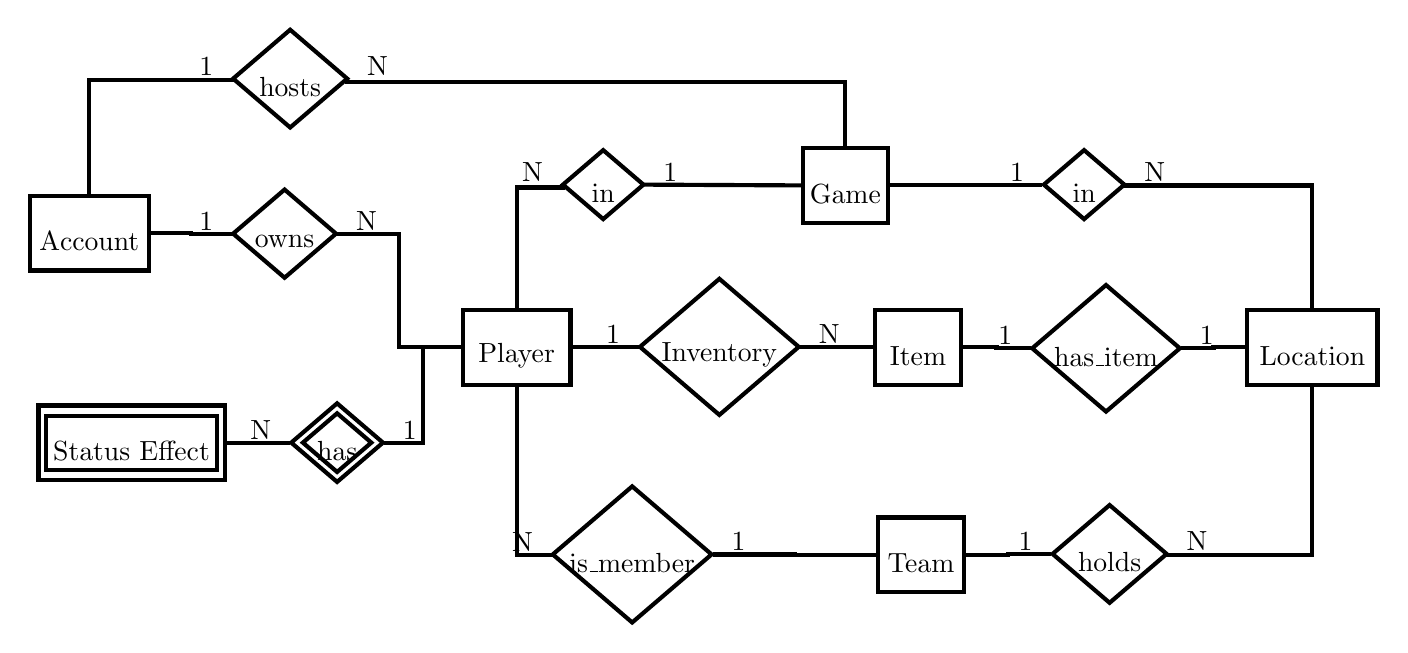
\begin{tikzpicture}
\pgftransformxscale{0.700000}
\pgftransformyscale{-1.000000}
\definecolor{dialinecolor}{rgb}{0.000000, 0.000000, 0.000000}
\pgfsetstrokecolor{dialinecolor}
\definecolor{dialinecolor}{rgb}{1.000000, 1.000000, 1.000000}
\pgfsetfillcolor{dialinecolor}
\definecolor{dialinecolor}{rgb}{1.000000, 1.000000, 1.000000}
\pgfsetfillcolor{dialinecolor}
\fill (-8.000000\du,-6.000000\du)--(-8.000000\du,-4.200000\du)--(-3.905000\du,-4.200000\du)--(-3.905000\du,-6.000000\du)--cycle;
\pgfsetlinewidth{0.100000\du}
\pgfsetdash{}{0pt}
\pgfsetmiterjoin
\definecolor{dialinecolor}{rgb}{0.000000, 0.000000, 0.000000}
\pgfsetstrokecolor{dialinecolor}
\draw (-8.000000\du,-6.000000\du)--(-8.000000\du,-4.200000\du)--(-3.905000\du,-4.200000\du)--(-3.905000\du,-6.000000\du)--cycle;
% setfont left to latex
\definecolor{dialinecolor}{rgb}{0.000000, 0.000000, 0.000000}
\pgfsetstrokecolor{dialinecolor}
\node at (-5.952500\du,-4.900000\du){Account};
\definecolor{dialinecolor}{rgb}{1.000000, 1.000000, 1.000000}
\pgfsetfillcolor{dialinecolor}
\fill (18.600000\du,-7.150000\du)--(18.600000\du,-5.350000\du)--(21.540000\du,-5.350000\du)--(21.540000\du,-7.150000\du)--cycle;
\pgfsetlinewidth{0.100000\du}
\pgfsetdash{}{0pt}
\pgfsetmiterjoin
\definecolor{dialinecolor}{rgb}{0.000000, 0.000000, 0.000000}
\pgfsetstrokecolor{dialinecolor}
\draw (18.600000\du,-7.150000\du)--(18.600000\du,-5.350000\du)--(21.540000\du,-5.350000\du)--(21.540000\du,-7.150000\du)--cycle;
% setfont left to latex
\definecolor{dialinecolor}{rgb}{0.000000, 0.000000, 0.000000}
\pgfsetstrokecolor{dialinecolor}
\node at (20.070000\du,-6.050000\du){Game};
\definecolor{dialinecolor}{rgb}{1.000000, 1.000000, 1.000000}
\pgfsetfillcolor{dialinecolor}
\fill (21.200000\du,1.750000\du)--(21.200000\du,3.550000\du)--(24.140000\du,3.550000\du)--(24.140000\du,1.750000\du)--cycle;
\pgfsetlinewidth{0.100000\du}
\pgfsetdash{}{0pt}
\pgfsetmiterjoin
\definecolor{dialinecolor}{rgb}{0.000000, 0.000000, 0.000000}
\pgfsetstrokecolor{dialinecolor}
\draw (21.200000\du,1.750000\du)--(21.200000\du,3.550000\du)--(24.140000\du,3.550000\du)--(24.140000\du,1.750000\du)--cycle;
% setfont left to latex
\definecolor{dialinecolor}{rgb}{0.000000, 0.000000, 0.000000}
\pgfsetstrokecolor{dialinecolor}
\node at (22.670000\du,2.850000\du){Team};
% setfont left to latex
\definecolor{dialinecolor}{rgb}{0.000000, 0.000000, 0.000000}
\pgfsetstrokecolor{dialinecolor}
\node[anchor=west] at (22.670000\du,2.650000\du){};
\definecolor{dialinecolor}{rgb}{1.000000, 1.000000, 1.000000}
\pgfsetfillcolor{dialinecolor}
\fill (13.000000\du,-2.360500\du)--(15.732500\du,-4.000000\du)--(18.465000\du,-2.360500\du)--(15.732500\du,-0.721000\du)--cycle;
\pgfsetlinewidth{0.100000\du}
\pgfsetdash{}{0pt}
\pgfsetmiterjoin
\definecolor{dialinecolor}{rgb}{0.000000, 0.000000, 0.000000}
\pgfsetstrokecolor{dialinecolor}
\draw (13.000000\du,-2.360500\du)--(15.732500\du,-4.000000\du)--(18.465000\du,-2.360500\du)--(15.732500\du,-0.721000\du)--cycle;
% setfont left to latex
\definecolor{dialinecolor}{rgb}{0.000000, 0.000000, 0.000000}
\pgfsetstrokecolor{dialinecolor}
\node[anchor=east] at (12.700000\du,-2.660500\du){1};
\definecolor{dialinecolor}{rgb}{0.000000, 0.000000, 0.000000}
\pgfsetstrokecolor{dialinecolor}
\node[anchor=west] at (18.765000\du,-2.660500\du){N};
\definecolor{dialinecolor}{rgb}{0.000000, 0.000000, 0.000000}
\pgfsetstrokecolor{dialinecolor}
\node at (15.732500\du,-2.160500\du){Inventory};
\definecolor{dialinecolor}{rgb}{1.000000, 1.000000, 1.000000}
\pgfsetfillcolor{dialinecolor}
\fill (21.100000\du,-3.250000\du)--(21.100000\du,-1.450000\du)--(24.040000\du,-1.450000\du)--(24.040000\du,-3.250000\du)--cycle;
\pgfsetlinewidth{0.100000\du}
\pgfsetdash{}{0pt}
\pgfsetmiterjoin
\definecolor{dialinecolor}{rgb}{0.000000, 0.000000, 0.000000}
\pgfsetstrokecolor{dialinecolor}
\draw (21.100000\du,-3.250000\du)--(21.100000\du,-1.450000\du)--(24.040000\du,-1.450000\du)--(24.040000\du,-3.250000\du)--cycle;
% setfont left to latex
\definecolor{dialinecolor}{rgb}{0.000000, 0.000000, 0.000000}
\pgfsetstrokecolor{dialinecolor}
\node at (22.570000\du,-2.150000\du){Item};
\definecolor{dialinecolor}{rgb}{1.000000, 1.000000, 1.000000}
\pgfsetfillcolor{dialinecolor}
\fill (26.500000\du,-2.325999\du)--(29.040000\du,-3.849999\du)--(31.580000\du,-2.325999\du)--(29.040000\du,-0.801999\du)--cycle;
\pgfsetlinewidth{0.100000\du}
\pgfsetdash{}{0pt}
\pgfsetmiterjoin
\definecolor{dialinecolor}{rgb}{0.000000, 0.000000, 0.000000}
\pgfsetstrokecolor{dialinecolor}
\draw (26.500000\du,-2.325999\du)--(29.040000\du,-3.849999\du)--(31.580000\du,-2.325999\du)--(29.040000\du,-0.801999\du)--cycle;
% setfont left to latex
\definecolor{dialinecolor}{rgb}{0.000000, 0.000000, 0.000000}
\pgfsetstrokecolor{dialinecolor}
\node[anchor=east] at (26.200000\du,-2.625999\du){1};
\definecolor{dialinecolor}{rgb}{0.000000, 0.000000, 0.000000}
\pgfsetstrokecolor{dialinecolor}
\node[anchor=west] at (31.880000\du,-2.625999\du){1};
\definecolor{dialinecolor}{rgb}{0.000000, 0.000000, 0.000000}
\pgfsetstrokecolor{dialinecolor}
\node at (29.040000\du,-2.125999\du){has\_item};
\definecolor{dialinecolor}{rgb}{1.000000, 1.000000, 1.000000}
\pgfsetfillcolor{dialinecolor}
\fill (33.900000\du,-3.250000\du)--(33.900000\du,-1.450000\du)--(38.380000\du,-1.450000\du)--(38.380000\du,-3.250000\du)--cycle;
\pgfsetlinewidth{0.100000\du}
\pgfsetdash{}{0pt}
\pgfsetmiterjoin
\definecolor{dialinecolor}{rgb}{0.000000, 0.000000, 0.000000}
\pgfsetstrokecolor{dialinecolor}
\draw (33.900000\du,-3.250000\du)--(33.900000\du,-1.450000\du)--(38.380000\du,-1.450000\du)--(38.380000\du,-3.250000\du)--cycle;
% setfont left to latex
\definecolor{dialinecolor}{rgb}{0.000000, 0.000000, 0.000000}
\pgfsetstrokecolor{dialinecolor}
\node at (36.140000\du,-2.150000\du){Location};
\definecolor{dialinecolor}{rgb}{1.000000, 1.000000, 1.000000}
\pgfsetfillcolor{dialinecolor}
\fill (27.200004\du,2.627500\du)--(29.162504\du,1.450000\du)--(31.125004\du,2.627500\du)--(29.162504\du,3.805000\du)--cycle;
\pgfsetlinewidth{0.100000\du}
\pgfsetdash{}{0pt}
\pgfsetmiterjoin
\definecolor{dialinecolor}{rgb}{0.000000, 0.000000, 0.000000}
\pgfsetstrokecolor{dialinecolor}
\draw (27.200004\du,2.627500\du)--(29.162504\du,1.450000\du)--(31.125004\du,2.627500\du)--(29.162504\du,3.805000\du)--cycle;
% setfont left to latex
\definecolor{dialinecolor}{rgb}{0.000000, 0.000000, 0.000000}
\pgfsetstrokecolor{dialinecolor}
\node[anchor=east] at (26.900004\du,2.327500\du){1};
\definecolor{dialinecolor}{rgb}{0.000000, 0.000000, 0.000000}
\pgfsetstrokecolor{dialinecolor}
\node[anchor=west] at (31.425004\du,2.327500\du){N};
\definecolor{dialinecolor}{rgb}{0.000000, 0.000000, 0.000000}
\pgfsetstrokecolor{dialinecolor}
\node at (29.162504\du,2.827500\du){holds};
\definecolor{dialinecolor}{rgb}{1.000000, 1.000000, 1.000000}
\pgfsetfillcolor{dialinecolor}
\fill (26.900004\du,-6.268999\du)--(28.285004\du,-7.099999\du)--(29.670004\du,-6.268999\du)--(28.285004\du,-5.437999\du)--cycle;
\pgfsetlinewidth{0.100000\du}
\pgfsetdash{}{0pt}
\pgfsetmiterjoin
\definecolor{dialinecolor}{rgb}{0.000000, 0.000000, 0.000000}
\pgfsetstrokecolor{dialinecolor}
\draw (26.900004\du,-6.268999\du)--(28.285004\du,-7.099999\du)--(29.670004\du,-6.268999\du)--(28.285004\du,-5.437999\du)--cycle;
% setfont left to latex
\definecolor{dialinecolor}{rgb}{0.000000, 0.000000, 0.000000}
\pgfsetstrokecolor{dialinecolor}
\node[anchor=east] at (26.600004\du,-6.568999\du){1};
\definecolor{dialinecolor}{rgb}{0.000000, 0.000000, 0.000000}
\pgfsetstrokecolor{dialinecolor}
\node[anchor=west] at (29.970004\du,-6.568999\du){N};
\definecolor{dialinecolor}{rgb}{0.000000, 0.000000, 0.000000}
\pgfsetstrokecolor{dialinecolor}
\node at (28.285004\du,-6.068999\du){in};
\definecolor{dialinecolor}{rgb}{1.000000, 1.000000, 1.000000}
\pgfsetfillcolor{dialinecolor}
\fill (-1.000000\du,-8.822500\du)--(0.962500\du,-10.000000\du)--(2.925000\du,-8.822500\du)--(0.962500\du,-7.645000\du)--cycle;
\pgfsetlinewidth{0.100000\du}
\pgfsetdash{}{0pt}
\pgfsetmiterjoin
\definecolor{dialinecolor}{rgb}{0.000000, 0.000000, 0.000000}
\pgfsetstrokecolor{dialinecolor}
\draw (-1.000000\du,-8.822500\du)--(0.962500\du,-10.000000\du)--(2.925000\du,-8.822500\du)--(0.962500\du,-7.645000\du)--cycle;
% setfont left to latex
\definecolor{dialinecolor}{rgb}{0.000000, 0.000000, 0.000000}
\pgfsetstrokecolor{dialinecolor}
\node[anchor=east] at (-1.300000\du,-9.122500\du){1};
\definecolor{dialinecolor}{rgb}{0.000000, 0.000000, 0.000000}
\pgfsetstrokecolor{dialinecolor}
\node[anchor=west] at (3.225000\du,-9.122500\du){N};
\definecolor{dialinecolor}{rgb}{0.000000, 0.000000, 0.000000}
\pgfsetstrokecolor{dialinecolor}
\node at (0.962500\du,-8.622500\du){hosts};
\definecolor{dialinecolor}{rgb}{1.000000, 1.000000, 1.000000}
\pgfsetfillcolor{dialinecolor}
\fill (6.900000\du,-3.250001\du)--(6.900000\du,-1.450001\du)--(10.610000\du,-1.450001\du)--(10.610000\du,-3.250001\du)--cycle;
\pgfsetlinewidth{0.100000\du}
\pgfsetdash{}{0pt}
\pgfsetmiterjoin
\definecolor{dialinecolor}{rgb}{0.000000, 0.000000, 0.000000}
\pgfsetstrokecolor{dialinecolor}
\draw (6.900000\du,-3.250001\du)--(6.900000\du,-1.450001\du)--(10.610000\du,-1.450001\du)--(10.610000\du,-3.250001\du)--cycle;
% setfont left to latex
\definecolor{dialinecolor}{rgb}{0.000000, 0.000000, 0.000000}
\pgfsetstrokecolor{dialinecolor}
\node at (8.755000\du,-2.150001\du){Player};
\definecolor{dialinecolor}{rgb}{1.000000, 1.000000, 1.000000}
\pgfsetfillcolor{dialinecolor}
\fill (-1.000000\du,-5.088000\du)--(0.770000\du,-6.150000\du)--(2.540000\du,-5.088000\du)--(0.770000\du,-4.026000\du)--cycle;
\pgfsetlinewidth{0.100000\du}
\pgfsetdash{}{0pt}
\pgfsetmiterjoin
\definecolor{dialinecolor}{rgb}{0.000000, 0.000000, 0.000000}
\pgfsetstrokecolor{dialinecolor}
\draw (-1.000000\du,-5.088000\du)--(0.770000\du,-6.150000\du)--(2.540000\du,-5.088000\du)--(0.770000\du,-4.026000\du)--cycle;
% setfont left to latex
\definecolor{dialinecolor}{rgb}{0.000000, 0.000000, 0.000000}
\pgfsetstrokecolor{dialinecolor}
\node[anchor=east] at (-1.300000\du,-5.388000\du){1};
\definecolor{dialinecolor}{rgb}{0.000000, 0.000000, 0.000000}
\pgfsetstrokecolor{dialinecolor}
\node[anchor=west] at (2.840000\du,-5.388000\du){N};
\definecolor{dialinecolor}{rgb}{0.000000, 0.000000, 0.000000}
\pgfsetstrokecolor{dialinecolor}
\node at (0.770000\du,-4.888000\du){owns};
\definecolor{dialinecolor}{rgb}{1.000000, 1.000000, 1.000000}
\pgfsetfillcolor{dialinecolor}
\fill (10.350000\du,-6.269000\du)--(11.735000\du,-7.100000\du)--(13.120000\du,-6.269000\du)--(11.735000\du,-5.438000\du)--cycle;
\pgfsetlinewidth{0.100000\du}
\pgfsetdash{}{0pt}
\pgfsetmiterjoin
\definecolor{dialinecolor}{rgb}{0.000000, 0.000000, 0.000000}
\pgfsetstrokecolor{dialinecolor}
\draw (10.350000\du,-6.269000\du)--(11.735000\du,-7.100000\du)--(13.120000\du,-6.269000\du)--(11.735000\du,-5.438000\du)--cycle;
% setfont left to latex
\definecolor{dialinecolor}{rgb}{0.000000, 0.000000, 0.000000}
\pgfsetstrokecolor{dialinecolor}
\node[anchor=east] at (10.050000\du,-6.569000\du){N};
\definecolor{dialinecolor}{rgb}{0.000000, 0.000000, 0.000000}
\pgfsetstrokecolor{dialinecolor}
\node[anchor=west] at (13.420000\du,-6.569000\du){1};
\definecolor{dialinecolor}{rgb}{0.000000, 0.000000, 0.000000}
\pgfsetstrokecolor{dialinecolor}
\node at (11.735000\du,-6.069000\du){in};
\pgfsetlinewidth{0.100000\du}
\pgfsetdash{}{0pt}
\pgfsetdash{}{0pt}
\pgfsetbuttcap
{
\definecolor{dialinecolor}{rgb}{0.000000, 0.000000, 0.000000}
\pgfsetfillcolor{dialinecolor}
% was here!!!
\definecolor{dialinecolor}{rgb}{0.000000, 0.000000, 0.000000}
\pgfsetstrokecolor{dialinecolor}
\draw (13.120000\du,-6.269000\du)--(18.600000\du,-6.250000\du);
}
\definecolor{dialinecolor}{rgb}{1.000000, 1.000000, 1.000000}
\pgfsetfillcolor{dialinecolor}
\fill (10.000000\du,2.639500\du)--(12.732500\du,1.000000\du)--(15.465000\du,2.639500\du)--(12.732500\du,4.279000\du)--cycle;
\pgfsetlinewidth{0.100000\du}
\pgfsetdash{}{0pt}
\pgfsetmiterjoin
\definecolor{dialinecolor}{rgb}{0.000000, 0.000000, 0.000000}
\pgfsetstrokecolor{dialinecolor}
\draw (10.000000\du,2.639500\du)--(12.732500\du,1.000000\du)--(15.465000\du,2.639500\du)--(12.732500\du,4.279000\du)--cycle;
% setfont left to latex
\definecolor{dialinecolor}{rgb}{0.000000, 0.000000, 0.000000}
\pgfsetstrokecolor{dialinecolor}
\node[anchor=east] at (9.700000\du,2.339500\du){N};
\definecolor{dialinecolor}{rgb}{0.000000, 0.000000, 0.000000}
\pgfsetstrokecolor{dialinecolor}
\node[anchor=west] at (15.765000\du,2.339500\du){1};
\definecolor{dialinecolor}{rgb}{0.000000, 0.000000, 0.000000}
\pgfsetstrokecolor{dialinecolor}
\node at (12.732500\du,2.839500\du){is\_member};
\definecolor{dialinecolor}{rgb}{1.000000, 1.000000, 1.000000}
\pgfsetfillcolor{dialinecolor}
\fill (-7.700000\du,-0.949999\du)--(-7.700000\du,0.850001\du)--(-1.295000\du,0.850001\du)--(-1.295000\du,-0.949999\du)--cycle;
\pgfsetlinewidth{0.100000\du}
\pgfsetdash{}{0pt}
\pgfsetmiterjoin
\definecolor{dialinecolor}{rgb}{0.000000, 0.000000, 0.000000}
\pgfsetstrokecolor{dialinecolor}
\draw (-7.700000\du,-0.949999\du)--(-7.700000\du,0.850001\du)--(-1.295000\du,0.850001\du)--(-1.295000\du,-0.949999\du)--cycle;
\definecolor{dialinecolor}{rgb}{0.000000, 0.000000, 0.000000}
\pgfsetstrokecolor{dialinecolor}
\draw (-7.450000\du,-0.699999\du)--(-7.450000\du,0.600001\du)--(-1.545000\du,0.600001\du)--(-1.545000\du,-0.699999\du)--cycle;
% setfont left to latex
\definecolor{dialinecolor}{rgb}{0.000000, 0.000000, 0.000000}
\pgfsetstrokecolor{dialinecolor}
\node at (-4.497500\du,0.150001\du){Status Effect};
\definecolor{dialinecolor}{rgb}{1.000000, 1.000000, 1.000000}
\pgfsetfillcolor{dialinecolor}
\fill (1.000000\du,-0.053500\du)--(2.577500\du,-1.000000\du)--(4.155000\du,-0.053500\du)--(2.577500\du,0.893000\du)--cycle;
\pgfsetlinewidth{0.100000\du}
\pgfsetdash{}{0pt}
\pgfsetmiterjoin
\definecolor{dialinecolor}{rgb}{0.000000, 0.000000, 0.000000}
\pgfsetstrokecolor{dialinecolor}
\draw (1.000000\du,-0.053500\du)--(2.577500\du,-1.000000\du)--(4.155000\du,-0.053500\du)--(2.577500\du,0.893000\du)--cycle;
\definecolor{dialinecolor}{rgb}{0.000000, 0.000000, 0.000000}
\pgfsetstrokecolor{dialinecolor}
\draw (1.400000\du,-0.053500\du)--(2.577500\du,-0.760000\du)--(3.755000\du,-0.053500\du)--(2.577500\du,0.653000\du)--cycle;
% setfont left to latex
\definecolor{dialinecolor}{rgb}{0.000000, 0.000000, 0.000000}
\pgfsetstrokecolor{dialinecolor}
\node[anchor=east] at (0.700000\du,-0.353500\du){N};
\definecolor{dialinecolor}{rgb}{0.000000, 0.000000, 0.000000}
\pgfsetstrokecolor{dialinecolor}
\node[anchor=west] at (4.455000\du,-0.353500\du){1};
\definecolor{dialinecolor}{rgb}{0.000000, 0.000000, 0.000000}
\pgfsetstrokecolor{dialinecolor}
\node at (2.577500\du,0.146500\du){has};
\pgfsetlinewidth{0.100000\du}
\pgfsetdash{}{0pt}
\pgfsetdash{}{0pt}
\pgfsetmiterjoin
\pgfsetbuttcap
{
\definecolor{dialinecolor}{rgb}{0.000000, 0.000000, 0.000000}
\pgfsetfillcolor{dialinecolor}
% was here!!!
{\pgfsetcornersarced{\pgfpoint{0.000000\du}{0.000000\du}}\definecolor{dialinecolor}{rgb}{0.000000, 0.000000, 0.000000}
\pgfsetstrokecolor{dialinecolor}
\draw (20.070000\du,-7.150000\du)--(20.070000\du,-8.749106\du)--(2.925000\du,-8.749106\du)--(2.925000\du,-8.822500\du);
}}
\pgfsetlinewidth{0.100000\du}
\pgfsetdash{}{0pt}
\pgfsetdash{}{0pt}
\pgfsetmiterjoin
\pgfsetbuttcap
{
\definecolor{dialinecolor}{rgb}{0.000000, 0.000000, 0.000000}
\pgfsetfillcolor{dialinecolor}
% was here!!!
{\pgfsetcornersarced{\pgfpoint{0.000000\du}{0.000000\du}}\definecolor{dialinecolor}{rgb}{0.000000, 0.000000, 0.000000}
\pgfsetstrokecolor{dialinecolor}
\draw (-1.000000\du,-8.822500\du)--(-1.000000\du,-8.799106\du)--(-5.952500\du,-8.799106\du)--(-5.952500\du,-6.000000\du);
}}
\pgfsetlinewidth{0.100000\du}
\pgfsetdash{}{0pt}
\pgfsetdash{}{0pt}
\pgfsetmiterjoin
\pgfsetbuttcap
{
\definecolor{dialinecolor}{rgb}{0.000000, 0.000000, 0.000000}
\pgfsetfillcolor{dialinecolor}
% was here!!!
{\pgfsetcornersarced{\pgfpoint{0.000000\du}{0.000000\du}}\definecolor{dialinecolor}{rgb}{0.000000, 0.000000, 0.000000}
\pgfsetstrokecolor{dialinecolor}
\draw (-1.000000\du,-5.088000\du)--(-2.452500\du,-5.088000\du)--(-2.452500\du,-5.100000\du)--(-3.905000\du,-5.100000\du);
}}
\pgfsetlinewidth{0.100000\du}
\pgfsetdash{}{0pt}
\pgfsetdash{}{0pt}
\pgfsetmiterjoin
\pgfsetbuttcap
{
\definecolor{dialinecolor}{rgb}{0.000000, 0.000000, 0.000000}
\pgfsetfillcolor{dialinecolor}
% was here!!!
{\pgfsetcornersarced{\pgfpoint{0.000000\du}{0.000000\du}}\definecolor{dialinecolor}{rgb}{0.000000, 0.000000, 0.000000}
\pgfsetstrokecolor{dialinecolor}
\draw (2.540000\du,-5.088000\du)--(4.720000\du,-5.088000\du)--(4.720000\du,-2.350001\du)--(6.900000\du,-2.350001\du);
}}
\pgfsetlinewidth{0.100000\du}
\pgfsetdash{}{0pt}
\pgfsetdash{}{0pt}
\pgfsetmiterjoin
\pgfsetbuttcap
{
\definecolor{dialinecolor}{rgb}{0.000000, 0.000000, 0.000000}
\pgfsetfillcolor{dialinecolor}
% was here!!!
{\pgfsetcornersarced{\pgfpoint{0.000000\du}{0.000000\du}}\definecolor{dialinecolor}{rgb}{0.000000, 0.000000, 0.000000}
\pgfsetstrokecolor{dialinecolor}
\draw (10.350000\du,-6.269000\du)--(10.350000\du,-6.199108\du)--(8.755000\du,-6.199108\du)--(8.755000\du,-3.299591\du);
}}
\pgfsetlinewidth{0.100000\du}
\pgfsetdash{}{0pt}
\pgfsetdash{}{0pt}
\pgfsetmiterjoin
\pgfsetbuttcap
{
\definecolor{dialinecolor}{rgb}{0.000000, 0.000000, 0.000000}
\pgfsetfillcolor{dialinecolor}
% was here!!!
{\pgfsetcornersarced{\pgfpoint{0.000000\du}{0.000000\du}}\definecolor{dialinecolor}{rgb}{0.000000, 0.000000, 0.000000}
\pgfsetstrokecolor{dialinecolor}
\draw (6.849535\du,-2.350001\du)--(5.527070\du,-2.350001\du)--(5.527070\du,-0.053500\du)--(4.204606\du,-0.053500\du);
}}
\pgfsetlinewidth{0.100000\du}
\pgfsetdash{}{0pt}
\pgfsetdash{}{0pt}
\pgfsetmiterjoin
\pgfsetbuttcap
{
\definecolor{dialinecolor}{rgb}{0.000000, 0.000000, 0.000000}
\pgfsetfillcolor{dialinecolor}
% was here!!!
{\pgfsetcornersarced{\pgfpoint{0.000000\du}{0.000000\du}}\definecolor{dialinecolor}{rgb}{0.000000, 0.000000, 0.000000}
\pgfsetstrokecolor{dialinecolor}
\draw (12.952405\du,-2.360500\du)--(11.806435\du,-2.360500\du)--(11.806435\du,-2.350001\du)--(10.660465\du,-2.350001\du);
}}
\pgfsetlinewidth{0.100000\du}
\pgfsetdash{}{0pt}
\pgfsetdash{}{0pt}
\pgfsetmiterjoin
\pgfsetbuttcap
{
\definecolor{dialinecolor}{rgb}{0.000000, 0.000000, 0.000000}
\pgfsetfillcolor{dialinecolor}
% was here!!!
{\pgfsetcornersarced{\pgfpoint{0.000000\du}{0.000000\du}}\definecolor{dialinecolor}{rgb}{0.000000, 0.000000, 0.000000}
\pgfsetstrokecolor{dialinecolor}
\draw (21.049629\du,-2.350000\du)--(19.781112\du,-2.350000\du)--(19.781112\du,-2.360500\du)--(18.512595\du,-2.360500\du);
}}
\pgfsetlinewidth{0.100000\du}
\pgfsetdash{}{0pt}
\pgfsetdash{}{0pt}
\pgfsetmiterjoin
\pgfsetbuttcap
{
\definecolor{dialinecolor}{rgb}{0.000000, 0.000000, 0.000000}
\pgfsetfillcolor{dialinecolor}
% was here!!!
{\pgfsetcornersarced{\pgfpoint{0.000000\du}{0.000000\du}}\definecolor{dialinecolor}{rgb}{0.000000, 0.000000, 0.000000}
\pgfsetstrokecolor{dialinecolor}
\draw (24.090371\du,-2.350000\du)--(25.271496\du,-2.350000\du)--(25.271496\du,-2.325999\du)--(26.452622\du,-2.325999\du);
}}
\pgfsetlinewidth{0.100000\du}
\pgfsetdash{}{0pt}
\pgfsetdash{}{0pt}
\pgfsetmiterjoin
\pgfsetbuttcap
{
\definecolor{dialinecolor}{rgb}{0.000000, 0.000000, 0.000000}
\pgfsetfillcolor{dialinecolor}
% was here!!!
{\pgfsetcornersarced{\pgfpoint{0.000000\du}{0.000000\du}}\definecolor{dialinecolor}{rgb}{0.000000, 0.000000, 0.000000}
\pgfsetstrokecolor{dialinecolor}
\draw (21.590371\du,-6.250000\du)--(24.220066\du,-6.250000\du)--(24.220066\du,-6.268999\du)--(26.849760\du,-6.268999\du);
}}
\pgfsetlinewidth{0.100000\du}
\pgfsetdash{}{0pt}
\pgfsetdash{}{0pt}
\pgfsetmiterjoin
\pgfsetbuttcap
{
\definecolor{dialinecolor}{rgb}{0.000000, 0.000000, 0.000000}
\pgfsetfillcolor{dialinecolor}
% was here!!!
{\pgfsetcornersarced{\pgfpoint{0.000000\du}{0.000000\du}}\definecolor{dialinecolor}{rgb}{0.000000, 0.000000, 0.000000}
\pgfsetstrokecolor{dialinecolor}
\draw (36.140000\du,-3.250000\du)--(36.140000\du,-6.249108\du)--(29.670004\du,-6.249108\du)--(29.670004\du,-6.268999\du);
}}
\pgfsetlinewidth{0.100000\du}
\pgfsetdash{}{0pt}
\pgfsetdash{}{0pt}
\pgfsetmiterjoin
\pgfsetbuttcap
{
\definecolor{dialinecolor}{rgb}{0.000000, 0.000000, 0.000000}
\pgfsetfillcolor{dialinecolor}
% was here!!!
{\pgfsetcornersarced{\pgfpoint{0.000000\du}{0.000000\du}}\definecolor{dialinecolor}{rgb}{0.000000, 0.000000, 0.000000}
\pgfsetstrokecolor{dialinecolor}
\draw (31.627378\du,-2.325999\du)--(32.738549\du,-2.325999\du)--(32.738549\du,-2.350000\du)--(33.849721\du,-2.350000\du);
}}
\pgfsetlinewidth{0.100000\du}
\pgfsetdash{}{0pt}
\pgfsetdash{}{0pt}
\pgfsetmiterjoin
\pgfsetbuttcap
{
\definecolor{dialinecolor}{rgb}{0.000000, 0.000000, 0.000000}
\pgfsetfillcolor{dialinecolor}
% was here!!!
{\pgfsetcornersarced{\pgfpoint{0.000000\du}{0.000000\du}}\definecolor{dialinecolor}{rgb}{0.000000, 0.000000, 0.000000}
\pgfsetstrokecolor{dialinecolor}
\draw (21.149629\du,2.650000\du)--(18.331112\du,2.650000\du)--(18.331112\du,2.639500\du)--(15.512595\du,2.639500\du);
}}
\pgfsetlinewidth{0.100000\du}
\pgfsetdash{}{0pt}
\pgfsetdash{}{0pt}
\pgfsetmiterjoin
\pgfsetbuttcap
{
\definecolor{dialinecolor}{rgb}{0.000000, 0.000000, 0.000000}
\pgfsetfillcolor{dialinecolor}
% was here!!!
{\pgfsetcornersarced{\pgfpoint{0.000000\du}{0.000000\du}}\definecolor{dialinecolor}{rgb}{0.000000, 0.000000, 0.000000}
\pgfsetstrokecolor{dialinecolor}
\draw (24.190371\du,2.650000\du)--(25.672778\du,2.650000\du)--(25.672778\du,2.627500\du)--(27.155184\du,2.627500\du);
}}
\pgfsetlinewidth{0.100000\du}
\pgfsetdash{}{0pt}
\pgfsetdash{}{0pt}
\pgfsetmiterjoin
\pgfsetbuttcap
{
\definecolor{dialinecolor}{rgb}{0.000000, 0.000000, 0.000000}
\pgfsetfillcolor{dialinecolor}
% was here!!!
{\pgfsetcornersarced{\pgfpoint{0.000000\du}{0.000000\du}}\definecolor{dialinecolor}{rgb}{0.000000, 0.000000, 0.000000}
\pgfsetstrokecolor{dialinecolor}
\draw (-1.244603\du,-0.049999\du)--(-0.147104\du,-0.049999\du)--(-0.147104\du,-0.053500\du)--(0.950394\du,-0.053500\du);
}}
\pgfsetlinewidth{0.100000\du}
\pgfsetdash{}{0pt}
\pgfsetdash{}{0pt}
\pgfsetmiterjoin
\pgfsetbuttcap
{
\definecolor{dialinecolor}{rgb}{0.000000, 0.000000, 0.000000}
\pgfsetfillcolor{dialinecolor}
% was here!!!
{\pgfsetcornersarced{\pgfpoint{0.000000\du}{0.000000\du}}\definecolor{dialinecolor}{rgb}{0.000000, 0.000000, 0.000000}
\pgfsetstrokecolor{dialinecolor}
\draw (8.755000\du,-1.399820\du)--(8.755000\du,2.650885\du)--(10.000000\du,2.650885\du)--(10.000000\du,2.639500\du);
}}
\pgfsetlinewidth{0.100000\du}
\pgfsetdash{}{0pt}
\pgfsetdash{}{0pt}
\pgfsetmiterjoin
\pgfsetbuttcap
{
\definecolor{dialinecolor}{rgb}{0.000000, 0.000000, 0.000000}
\pgfsetfillcolor{dialinecolor}
% was here!!!
{\pgfsetcornersarced{\pgfpoint{0.000000\du}{0.000000\du}}\definecolor{dialinecolor}{rgb}{0.000000, 0.000000, 0.000000}
\pgfsetstrokecolor{dialinecolor}
\draw (36.140000\du,-1.399820\du)--(36.140000\du,2.650885\du)--(31.125004\du,2.650885\du)--(31.125004\du,2.627500\du);
}}
\end{tikzpicture}
  
  \caption{ER Diagram.}
  \label{fig:ER}
\end{figure}

\paragraph{Account}
The Account entity represent the users in the system. An account can host games represented by the host relation and take part in games represented as owning a player in a particular game.

\paragraph{Player}
This entity represents a user playing in a game. A player can hold items, have status effects and be a member of a team represented by Inventory, has(Status Effect) and Team(is\_member) respectively. The player entity also contains score and location etc. for a particular player in a game.

\paragraph{Game}
This entity represent games either \textit{starting up}, \textit{in progress} or \textit{ended}.

\paragraph{Status Effect}
Effects on a player is represented by this entity. An effect could be \textit{disabled until time} on a particular player. Status Effects have an effect type which the game logic is responsible for defining.

\paragraph{Team}
Players can be members of teams in a game, though a player is not required to be on a team to allow free for all game modes.

\paragraph{Item}
Items represent any object in the inventory of players or on a location in the game world. Items can be anything from objects players can "pick up" to a capture-able area in the game world. The attributes and behavior of items are defined by game logic.

\paragraph{Location}
A location is an item in the game world that can belong to a team. To own a location, a team must take it first.






\section{Implementation}
The implementation of the server is described in this section. The section contains implementation details of the Dispatcher, Logic Layer and Data Layer.\\

The implementation is based on the choices made in the framework design from \cref{sec:desFram}
%Dispatcher service
\subsection{Dispatcher Service}
The Dispatcher Service handles communication with the client through TCP/IP. We chose this protocol because it ensures data are correct upon arrival at the server, it is offered as library in the C\# programming language that we use to program our framework and we have minor experience using it from previous projects. 

Just like TCP/IP is offered in our programming language, there is also a library for Asynchronous IO. 

We wanted the implementation of our Dispatcher Service to be quick because we wanted to work on more specific framework flexibility and functionality. Network communication has been done in many other applications and we did not want to spend a long time on something that can be copied from others and does not differ far from other implementations. 

\subsubsection{Asynchronous IO}
\label{sec:asyncImplementation}
We decided to base our asynchronous IO implementation on \cite{asynh-imlp}. The implementation consist of a few method to handle async OI, these are \texttt{StartListening}, \texttt{AcceptCallback}, \texttt{ReadCallback} and \texttt{Send}. \texttt{StartListening} is responsible for listening for sockets connections and when a connection is established a AsyncCallback(part of the .net threading library) is made with \texttt{AcceptCallback} to process the incoming data. \texttt{AcceptCallback} prepares for receiving data then calls \texttt{ReadCallback}. \texttt{ReadCallback} reads data from the socket until an end of file tag is read at which point the data is parsed on to the dispatcher. Finally \texttt{Send} is used to send the result of the request back to the client.  %http://msdn.microsoft.com/en-us/library/fx6588te%28v=vs.110%29.aspx
\subsection{Dispatcher}
\label{chap:dispImplementation}
The Dispatcher has been implemented as conditional checking for methods. It will statically look for the methods that exist in the Admin class, and call the right method accordingly. The Dispatcher searches for a method call by checking if the XML contains each method name.

The Dispatcher handles all calls to the game thread by looking for the XML-tag \textit{<GameId>}. Throughout the framework, this XML-tag signals that the current clients requests should be handed over to the game thread\fixme{Dette skal skrives meget tydeligere, uklart hvordan det bliver handled}. The Dispatcher then dynamically invokes the correct method on the specified game thread, provided by the \textit{<GameId>} in the XML. 

\begin{lstlisting}[caption={Dynamically invoking methods on game threads}, language=C]
//Locate method call in XML sent from client
string methodCall = xh.GetMethodCallFromXML(xml);
object[] methodParams = {xml};

//Invoke method on correct game thread
Type type = typeof(GameThread);
MethodInfo method = type.GetMethod(methodCall);
GameThread c = AsynchronousSocketListener.gameThreadPool.GetGameInstance(xh.GetGameIdFromXML(xml));
string result = (string)method.Invoke(c, methodParams);
\end{lstlisting}

The Dispatcher will always return a XML-string to the Async IO.


%Logic Layer
\subsection{Logic Layer}
In this section we will describe the implementation of the Logic Layer as the game developed alongside the architecture. The Admin, Event Timer modules and Game Thread are implemented as an \texttt{Admin}, \texttt{EventTimer} and \texttt{GameThread} class respectively. Additionally XML helper classes \texttt{XMLBuilder} and \texttt{XMLHandler} will be covered.

Since we developed a game alongside our framework, we implemented our own version of the Game Thread. We realised that XML would become a big part of the framework, and we would be writing the same code in multiple places if we did not implement a generic way to handle and build the XML communication interface. Additionally, we could handle conversion from strings of characters to the correct type in the XML handler. 

The Event Timer has been implemented as framework functionality and it works as intended, although we did use it in the game we developed. The implementation allows the user to specify any event in the Game Event class and call it upon a Game Thread. 

The framework allows the use of items, which we in our game designed and developed as weapons. However, the user of the framework can consider in whichever way desired. Our game has implemented a Weapon class, which specifies a list of weapons to be used in the game. If you wish to store a harmful shot hitting a player, reducing the health-points of the player, the database offers the use of \textit{Status Effect} to store this for later use. Since the implementation of Items is game specific, we do not explain our implementation of weapons further.

\subsubsection{Admin}
\label{sec:adminimpl}
The Admin class handles requests from the client that can be classified as not game specific. These are requests like:
\begin{itemize}
\item \textit{VerifiyAccount} handles login-requests from the client.
\item \textit{CreateGame} handles requests to create and start a new game.
\end{itemize}

The Admin will handle these requests by querying the database through the Data Layer, more specific the DBController class. The database will then return the desired data that can be used for something like administrative logic for login, the information in this case being the password for a given username. These logical computations will be available in the Admin class, alongside functionality to fetch all active games stored in the database. We made this functionality, because we want to avoid asking all active Game Threads to respond to a client request looking for all active games. This would be bad design considering our desire to make a scalable framework, imagine if thousands of users requests to see the list of active games. 




\subsubsection{Event Timer}
\label{sec:eventtimerimpl}
The Event Timer is started when the server launches. It runs in its own thread and it enters an infinite loop where it loops over Game Events. For every iteration in the loop, the Event Timer checks all Game Events in the list to see whether the current time is past the timestamp for the Game Event. 

All Game Events are assigned a timestamp upon creation. The Event Timer iterates through the list of Game Events, and checks the timestamp by calling the method \textit{GetTriggerTimestamp()} and compares it to the current time. If the timestamp value is less than the current time (in other words, the event trigger threshold has been passed), the Game Event is triggered by calling the \textit{RunGameEvent()} method assigned to each Game Event. 

The Event Timer provides a method called \textit{AddGameEvent()}, which allows addition of new game events to its internal list of Game Events.

After a Game Event has been triggered, it is removed from the list in the Event Timer. This is done using the native \textit{RemoveAt()} method which are a part of lists in C\#.

The Event Timer class is a part of the framework, whereas the Game Event, described in \cref{subsec:geventImpl} is not.

\subsubsection{Game Event}\label{subsec:geventImpl}
The Game Event is implemented as a ``container'' for information about Game Events. It has a constructor which initializes variables gameId, eventType and triggerTimestamp. The rest of the class simply consists of getters for these variables. The getters are used by the Event Timer, described in \cref{subsec:eventtimerimpl}. Instances of the Game Event class are game specific, which means that each of the instantiated Game Events belong to a game, and are therefore not part of the framework. The user of the framework can code any desired Game Events into this class.
\subsection{Implementation of Game Thread}
\label{sec:gamethreadimpl}
Each active game is running as an instance of the game thread class on a separate thread on the server. The thread will not perform any actions on its own, but sits idle until another part of the server initializes a call to it. The parts of the server which can perform a call to a game thread are Admin, Dispatcher, GlobalTimerThread. Further explanation can be seen in design of game thread\ref{designgamethread}. 

The game thread has to handle a lot of different calls from different parts of the server, however it does not hold any game specific information itself. Every change to a game state, locations, events, actions, etc, will change the state of a game in the database. Therefore the game thread acts as a connection between information stored in the database and the requests made by the client.

All public methods in the game thread receives a string as parameter, because the methods within game thread handles the XML by itself. This XML is made by the client and contains all parameters the method needs. Each method in the game thread can then use the XMLhandler to pull out the desired data and convert it to the right type. The method hereby receives an object as the right type which it can proceed to work with.

The game thread contains private methods for handling private calculations. An example of this could be the method called \textit{PlaceObjectsOnRectangularBoard}, which is called when creating a game. It takes an argument for the number of objects to place on the board, the south-east boundary coordinate, the north-west boundary coordinate, and the collision radius to keep between the objects to handle the spread on the board. 



\subsubsection{XML handler}
\label{sec:xmlhandlerimpl}
To handle incoming requests from clients, a component was needed to read and translate the XML formatted strings that communication is based on. This resulted in the \textit{XMLhandler} class. The class has many methods, but is simple to use. Given any valid string of XML, the XML handler returns an object of correct type given the value stored in the XML. An example is the method \textit{GetGameIdFromXML}, it will extract an integer with a value specified in the XML. The method call will convert this from string to integer and return it. 

The XML handler is placed in the \textit{Logic Layer}. It is possible to argue for this class to be made static. The XML handler read the XML-interface between the client and the server, it is therefore a specific piece of game logic.  Specific pieces of game logic cannot be considered as part of the framework, hereby the XML handler is not.

All methods are designed to handle individual requests. Given that the type of request is now known, the relevant method can now be used to decode and convert values stored within the XML string into readable formats. It can hereafter be used as valid objects of correct type in the code.

The XML handler encapsulates all value extraction from XML. If a given XML-tag cannot be handled by the XML handler, it is easy to create a new method that handles this given part. The XML handler does not perform any logical calculation.
\subsubsection{XML Builder}
\label{sec:xmlbuilderimpl}
To construct responds to the incoming requests from clients, a component was needed to construct an XML formatted string. The result is the \textit{XMLbuilder} class. This class has one or two respond-messages per method that can be called on the server. Some has just got a single response-messages, because the only thing that changes is the parameters. Others have two respond-messages because they can out different results, e.g. a login-request can either be successful or fail. 

The XML builder is placed in the \textit{Logic Layer} because every response-message is specific for a piece of the game logic placed in the Game Thread. It is regarded as a part of the framework, but it has been used to develop the corresponding game and that can be seen in this class. The XML builder is not a necessary part to create, all response-message can be coded into the corresponding methods but it will affect the readability of the code and cluster a lot of string building into possibly complex methods. We chose to isolate the string building and created a separate class.

The \textit{XMLbuilder} is structured with a stringbuilder in each method. All methods for XML-building are formatted the same way in the code. If a XML-tag contains more information than an attribute, it will be split into a start-tag on one line, and an end-tag on another line. In between can be one or more tags, but if it only contains an attribute it will be a single line containing the start-tag, the attribute-value, and the end-tag. This makes the code easily readable when searching for the XML-formatting for a respond-message. 

The XML builder is compact and encapsulates all response-message very well. The class needs instantiation to be used, whereas it could arguably be more correct to make it as a static class. It is easy to create a new response-message, because already existing messages can be seen in the class.

We have two different standard formats for the XML strings. The first is a method call with attributes - the method name is used as an encapsulation with attributes as tags within. An example could be the response from the client entering a lobby. The response is encapsulated in the tags <Lobbyinfo></lobbyinfo>, with tags like <HostId> and <GameAlias>. The other standard format is a message from the server. An example could be the response to a login from the client. The response would be encapsulated in <Login></Login>, and contains a single tag called <Valid> with the value either true or false depending on the databases response.


%Data Layer
\subsection{Data Layer}
As described in \Cref{sec:server} the game treads and the admin class relies on a Data Mapper to handle communication with the database. The Data Mapper is based on the data mapper patten \fxwarning{ref WE bog}. The benefit of this is that the logic layer does not have to worry about the underlying database structure.
\subsubsection{Data Mapper} \label{sec:dbImplementation}
Handles reads, inserts, updates and deletes from the database. This is achieved by the exchange of domain objects between the logic layer and the data layer.
An example of this could be the Admin class requesting a list of all active games, the method for this takes no parameters, performs a lookup in game table, convert the result to domains objects and returns them as a list.
Another example could be a request for the a games a particular Account is taking part in. With the account id as parameter, the mapper performs lookups in the game and player (plays relation in the ER diagram \Cref{fig:ER}) tables, then converts it to a list of games.


\subsubsection{Domain Object} 
In order to represent the database in the logic layer we use Domain Objects. The domain objects are split into classes corresponding to tables in the database, though they do contain optional information based on foreign keys to other tables. An example could be a player domain object can contain information from the status effect table as well as the player table.



\subsection{Evaluation of Implementation}


%section test
\section{Test}
The aim of the project is to create a good base on which multiplayer games can easily be created. It is therefore desirable that the server is stable and able to handle a decent number of games at the same time without significant response time. More specifically we want a single server to be able to host as many games as possible without surpassing an average response time of 1000ms. Additionally we want to locate possible bottlenecks in the code, by recording the run time of each API call. This can be tested using a black-box testing.

The Python scripts used to test the server can be found in the folder named Test with the rest of the source code.\fixme{ret i forhold til hvor det ligger}

\subsection{Test Setup}
\label{sec:testSetup}
The test is done by simulating users through Python scripts: One for simulating a number of active games with the purpose of creating some artificial server load, and one for making single API calls and collecting data.

The first script creates server load by spawning a thread per desired game. Each thread creates a game, makes relevant API calls for the duration of the test, and finally it deletes the game. Each thread simulates very busy games with 2 API calls per second. 

The other script makes a single API call a number\fxfatal{what number?} of times, collects the run time for each call and finally calculates the mean and standard deviation. Because the goal is to stay on a run time under 1000ms, the number of calls taking more than this is also recorded.

Each script is run on seperate computers, to be sure the extra processing power needed to handle the game threats does not influence the test results. 

%The following API calls are used in the test:
%\begin{itemize}
%\item Login
%\item Create game
%\item Delete game
%\item Join game
%\item Leave game
%\item Change location
%\item Invite player
%\item List public games
%\item List joined games
%\item Get game info
%\item Shoot
%\end{itemize}

\subsection{Test Results}
<Results and things we learned from the tests.>
%In table \cref{tab:testRes} the results from the test are shown\fixme{Just latency test?}. Each test was perfomed with half a second interval.


\renewcommand{\arraystretch}{1.2}
\begin{table}
\label{tab:1}
\caption{Test with no load}
\centering
\begin{tabular}{|l|>{\raggedleft\arraybackslash}p{5em}|>{\raggedleft\arraybackslash}p{5em}|>{\raggedleft\arraybackslash}p{5em}|>{\raggedleft\arraybackslash}p{5em}|}
	\hline  & \multicolumn{1}{p{5em}|}{Mean (sec)} & \multicolumn{1}{p{5em}|}{\# over limit} & \multicolumn{1}{p{5em}|}{\# timed out} \\ 
	\hline Login  & 0.0135 & 3 & 0 \\ 
	\hline Get public games  & 0.0118 & 2 & 0 \\ 
	\hline Get joined games  & 0.0565 & 10 & 1 \\ 
	\hline Create game  & 0.0131 & 1 & 0 \\ 
	\hline Join game  & 0.0118 & 2 & 0 \\ 
	\hline Get game info  & 0.0114 & 2 & 0 \\ 
	\hline Invite player  & 0.0100 & 1 & 0 \\ 
	\hline Change position  & 0.0097 & 0 & 1 \\ 
	\hline Shoot player  & 0.0168 & 3 & 0 \\ 
	\hline Leave game  & 0.0067 & 1 & 1 \\ 
	\hline Delete game  & 0.0102 & 0 & 0 \\ 
	\hline 
\end{tabular} 
\end{table}

\begin{table}
\label{tab:2}
\caption{Test with load}
\centering
\begin{tabular}{|l|>{\raggedleft\arraybackslash}p{5em}|>{\raggedleft\arraybackslash}p{5em}|>{\raggedleft\arraybackslash}p{5em}|>{\raggedleft\arraybackslash}p{5em}|}
	\hline  & \multicolumn{1}{p{5em}|}{Mean} & \multicolumn{1}{p{5em}|}{\# over limit} & \multicolumn{1}{p{5em}|}{\# timed out} \\ 
	\hline Login  & 0.3676 & 262 & 1 \\ 
	\hline Get public games  & 0.4825 & 328 & 0 \\ 
	\hline Get joined games  & 0.4959 & 353 & 0 \\ 
	\hline Create game  & 0.4143 & 306 & 0 \\ 
	\hline Join game  & 0.4096 & 289 & 0 \\ 
	\hline Get game info  & 0.4051 & 279 & 0 \\ 
	\hline Invite player  & 0.3752 & 273 & 0 \\ 
	\hline Change position  & 0.4050 & 276 & 0 \\ 
	\hline Shoot  & 0.3806 & 259 & 0 \\ 
	\hline Leave game  & 0.3814 & 253 & 0 \\ 	
	\hline Delete game  & 0.3721 & 299 & 0 \\ 
	\hline 
\end{tabular} 
\end{table}
\renewcommand{\arraystretch}{1}












%\subsubsection{Test}
%\subsubsection{Login}
%\subsubsection{Game creation}
%\subsubsection{Join game}
%\subsubsection{Leave game}
%\subsubsection{Update player location}
%\subsubsection{Edit player invites}
%\subsubsection{Invite player}
%\subsubsection{title}




%\subsection{Sources of Error}
%There are a number of factors that possibly affect to the accuracy of the tests.\\

%One of the main sources of error is found in the nature\fixme{Overkill at sige nature?} of the internet. The tests were performed on a small local network and connections were sometimes closed because there was a fallout in the network. The test script, which the spammer, described in \cref{sec:testSetup}, then reconnected as soon as possible to maintain the highest possible amount of stress on the victim server. 